\documentclass[10pt,conference]{IEEEtran}
\usepackage{graphicx}
\usepackage{mathtools}
\usepackage{multirow}
\usepackage{multicol}
\usepackage[justification=centering]{caption}
\usepackage{float}
\usepackage[table]{xcolor}
\usepackage{multirow}
\usepackage[english]{babel}
\usepackage[utf8]{inputenc}
\usepackage{algorithm}
\usepackage{algpseudocode}
\usepackage{array}
\usepackage{cite}
\usepackage{multicol}
\usepackage{lipsum}
\usepackage{mwe}
\usepackage{pstricks}
\usepackage[font=small,labelfont=bf]{caption}
\captionsetup{justification=centering,singlelinecheck=false}
\captionsetup[figure]{name={Fig.},labelsep=period}
\newcommand{\minus}{\scalebox{0.75}[1.0]{$-$}}



\usepackage{lipsum}% http://ctan.org/pkg/lipsum
% Header & Footer
\newcommand{\MYfooter}{\smash{
\hfil\parbox[t][\height][t]{\textwidth}{\centering \thepage}\hfil \hbox{}}}
\pagestyle{plain}
\makeatletter
\def\ps@IEEEtitlepagestyle{%
\def\@oddhead{\parbox[t][\height][t]{\textwidth}{\centering
2016 29th International Conference on VLSI Design and 2016 15th International Conference on Embedded Systems\\
\noindent\makebox[\linewidth]{\rule{\textwidth}{0.0pt}}}\hfil\hbox{}}%
\def\@oddfoot{ 978-1-4673-8700-2/16 \$31.00 \textcopyright 2016 IEEE\newline DOI 10.1109/VLSID.2016.60\leftmark\mbox{}}%
\def\@evenfoot{\MYfooter}}
%H&F end

\begin{document}

\title{Stochastic Number Generation with Few Inputs}

\author{\IEEEauthorblockN{Ritsuko Muguruma}
\IEEEauthorblockA{Graduate School of Information Science and Engineering
\\Ritsumeikan University, Shiga, Japan
\\Email: csharp@ngc.is.ritumei.ac.jp}
\and
\IEEEauthorblockN{Shigeru Yamashita}
\IEEEauthorblockA{College of Information Science and Engineering
\\Ritsumeikan University, Shiga, Japan
\\Email: ger@cs.ritsumei.ac.jp}
}

\maketitle

\begin{abstract}
Stochastic computing (SC) has been attracting great
attention because it has many potential advantages compared
with conventional computation on binary radix encoding. Very
recently, a general design method of designing Boolean circuits
(functions) to realize SC operations has been proposed. As a
central part of the method, we need to design a logic function such
that its output becomes one with a certain desired probability.
Also, to realize an SC arithmetic operation with a constant value,
in some situations we need to prepare a random (stochastic)
number with a desired probability from a set of predetermined
random sources. We can utilize the above-mentioned previous
method to prepare stochastic numbers by designing Boolean
circuits. The method assumes all the random sources become
one with the same probability $\frac{1}{2}$. In this paper, we investigate
a different framework where we assume different probabilities
of each random numbers in the predetermined sources. Then,
we can propose a method to make a stochastic number by using
much fewer random input sources than the existing method.
Our experimental result shows that the generated circuits by our
method also tend to be smaller than the ones by the previous
method.

\end{abstract}
\begin{IEEEkeywords} 
Stochastic Computing; Stochastic Number
\end{IEEEkeywords}

\section{Introduction}
\label{intro}
Stochastic computing (SC) is an unconventional paradigm to
realize arithmetic computation, where real values are encoded
as stochastic bit-streams \cite{two}. There has been a great interest
in the research for SC because many researches have revealed
two major advantages of SC over conventional computation
on binary radix encoding.
\par One of the major advantages of SC is that we can perform
(especially) arithmetic operations with very low circuit area,
power, and usually fast speed compared to the conventional
way of computation if we admit some errors. Thus, there seem
to be many potential applications that make SC attractive for
VLSI implementation [6]. Indeed, there has been proposed
various applications of SC (e.g., \cite{seven}, \cite{eleven}, \cite{fourteen}). Another good
property of SC is its strong tolerance to bit flip errors [4],
[8] because it uses a uniform-weight encoding, and thus a
single bit flip happened anyway in a bit-stream does not affect
the encoded value significantly. This property will probably
become more important in the future because we will face
more and more variation problems with the continued scaling
of CMOS technology.
\par
There have been many researches concerning the design
methodology of SC circuits \cite{one}, \cite{six}, \cite{nine}. Very recently, a new
design approach has been proposed \cite{fifteen}; the method generates
a combinatorial logic circuit that uses auxiliary random inputs
to realize SC operations. The method only makes an assumption
on the necessary input probabilities without any additional
assumptions on the underlying combinatorial circuits. As a
central part of the method, we need to design a logic function
whose output becomes one with a certain desired probability.
The method uses k auxiliary inputs that becomes one with
probability $\frac{1}
{2}$ to design such a target logic function. From a
different perspective, this design problem can be considered
as generating a bit-stream that becomes one with a target
probability by using given (possibly many) random bit-streams
whose probabilities to be one is fixed. Such a random bitstream
may be used as a constant input bit-stream in an SC
operation. For example, as we see in the next section, scaled
addition needs constant random inputs whose probability can
control the scale value.
\par
Random bit-streams with required probabilities can be
produced using pseudo-random number generators (PRNGs).
However, PRNGs essentially produce deterministic sequences
which could fail some statistical tests. Furthermore, they
require a large amount of hardware cost. Thus, there have
been some researches \cite{three}, \cite{ten}, \cite{twelve}, \cite{thirteen} that consider how
to design a circuit to generate a random bit-stream whose
probability can be arbitrary as we desired from a given set
of random physical sources, such as thermal noise in circuits,
radioactive decay, and Brownian motion, etc. Indeed, how to
produce a random bit-stream with a “target” probability should
be an important issue in SC circuit design methodology in
many aspects.

\par
In this paper, we propose a new method to design a circuit
whose output becomes one with a certain desired probability.
Compared to the above-mentioned method used in \cite{fifteen}, our
method needs much fewer number of auxiliary inputs. More
concretely, if we use $k$ auxiliary inputs, our method can
generate multiple random bit-streams that becomes one with
any probability of the form $l/2^{\frac{k(k+1)}{2}}$
with an arbitrary integer $l (0\leq l\leq2^{\frac{k(k+1)}{2}})$ whereas the previous method used in [15] needs $2^{\frac{k(k+1)}{2}}$ auxiliary inputs which is quadratically more than our method. The previous method assumes all the random inputs become one with the same probability $\frac{1} {2}$. Our idea is to use different kinds of random inputs whose probabilities to be one are $\frac{1}{2},\frac{1}{2^{2}},...,\frac{1}{2^{k}}$. Our proposed method can be directly used to derive a smaller SC circuit to produce some probabilities that are used in the general SC circuit synthesis method proposed in \cite{fifteen}.

\par
Note that our method as well as the previous method used
in \cite{fifteen} can produce many different probability at the same time
from a fixed set of random bit-streams. If we need only one
(or very few) bit-stream, we do not need such a method; we
just tune a random source to be a desired probability. But if we
need a lot of random bit-streams with different probabilities,
it should be better to use our method in many applications.
The rest of this paper is organized as follows: Section II
provides a background knowledge of SC as well as the general
SC circuit synthesis method proposed in \cite{fifteen}. Then Section III
formally describes our problem, followed by Section IV that
proposes our method to solve the problem more efficiently
compared to the previous work. The comparison between our
method and the method \cite{fifteen} is given in Section V. At last
Section VI concludes the paper with some future works.

\section{PRELIMINARIES AND PREVIOUS WORKS}
\label{prelims & prevs}
\subsection{Stochastic Computing}
In SC, a number is represented by a bit-stream in such
a way that the probability (ratio) of “1” in the bit-steam
is interpreted as the number itself \cite{two}. For example, a bit-
stream “00101000” represents
$\frac{1}{4}$
because there are two “1”
in the 8 bit-length. We will sometimes refer to bit-streams
of this type as
stochastic numbers
(SNs). We also call the
probability a stochastic number represent as its
value
. Thus
two bit-streams that contain “1” with the same probability
represent the same number, i.e., we say that the values of
the two stochastic numbers are the same. For example, both
“101100” and “01010110” represents
$\frac{1}{2}$
, i.e., the values of the
two stochastic numbers are both
$\frac{1}{2}$
. Generally speaking, we can
increase the
precision
of the represented number by making
the bit-stream longer.
\par
As shown in Fig. 1, we can generate an SN by comparing
a (constant) binary number and a random number generated
by \textit{Linear Feedback Shift Register} (LFSR), etc. If we can use
an ideal random number, the probability of getting 1 from
such an SN can be controlled by the constant binary number.
Thus, we can generate an SN representing any number as we
want. In the following,
$Prob(X = 1)$ means the probability of getting 1 from the binary string $X$.

\par
An issue we should consider is the obvious fact that an SN
can represent only a real value in the range of
$[0,1]$. If we need to perform operations on numbers out of the range, we
need to scale the inputs to fit into the range of
$[0,1]$, and then
we need to scale again the final results appropriately after the whole stochastic computation.

\subsection{Arithmetic Operations in Stochastic Computing}
Here, we briefly explain how basic arithmetic operations
can be done in SC. Indeed, many operations can be done with
very simple logic gates as we will see in the following.

In SC, we can perform the multiplication of two SNs by
simply inputting the two bit-streams to an AND gate as shown
in Fig. 2. If the two SNs,$A$ and $B$, are independent with each other, we have the following:
$Prob (C = 1) = Prob (A = 1) \times Prob (B = 1)$ . From this, it is easy to see that a simple
AND gate can be used as a
stochastic multiplier
. Indeed, in
the example as shown in Fig. 2, we can surely get the correct result:
$C = A \times B$ because  $Prob( A = 1) = \frac{4}{8}$ and $Prob( B = 1) = \frac{6}{8}$, and $Prob( C = 1) = \frac{3}{8}$.
\par
In SC, as shown in Fig. 3, we can perform the addition of two SNs by using a multiplexer and an appropriate \textit{scaling} operation if necessary. If an SN $S$ is independent from both the two SNs, $A$ and $B$, we have the following:
$Prob(C = 1) = Prob (S = 1) \times Prob(A = 1) + Prob(S = 0)\times Prob (B = 1) = s\cdot a + (1 \minus s)\cdot b$. Especially, when
$Prob(S = 1) = \frac{1}{2},Prob(C = 1) = \frac{1}{2} (a+b)$
. Thus, we get an SN
$C$ which represents a number for the $\frac{1}{2}$ -scaled addition result: $\frac{1}{2}(A+B)$. Indeed, in the example as shown in Fig. 3, $Prob(A = 1) = \frac{5}{8}$, $Prob(B = 1) = \frac{3}{8}$ , $Prob (S = 1) = \frac{4}{8}$ and $Prob(C =1) = \frac{4}{8}$. This means we can get the half-scaled addition results. We may need to scale the result to get the real addition result if necessary.

\subsection{A General Design of Stochastic Circuits}
A general design method of SC circuits has been proposed
very recently [15]. In this section, we briefly review the
method since our method can improve the method with respect
to the number of necessary random inputs.

\par
When we want to calculate an arithmetic function, first we
approximate the desired function with a multivariate polyno-
mial by Taylor expansion, etc. Such approximation is usually
acceptable in SC because we essentially allow some errors
when we use SC. Thus, when we design an SC circuit, we
try to realize a multivariate polynomial, but for simplicity, we
consider a multi-linear function in the following. This is also
justified because we can transform a multivariate polynomial
into a multi-linear function by introducing more variables, e.g.,
$x_i^{2}$ is transformed into $x_{i_1} \cdot x_{i_2}$ with the condition that $x_{i_1} = x_{i_2} = x_i$. Thus, we consider a multi-linear function $f(x_1,x_2,...,x_n)$ in this paper.

\par
Each input $x_i$ in a target multi-linear $f(x_1,x_2,...,x_n)$ is given as an SN $X_i$ that becomes 1 with probability $x_i$. This means that $(0 \leq  x_i \leq 1)$ should be satisfied. If we want the input value of $x_i$ to be out of the above rage, we scale the values of all the input variables and the output values of the function as well by scaling and/or adding some constant value to the output value.

\par
In conclusion, our essential task is to design a circuit to
realize a multi-linear function
$f(x_1,x_2,...,x_n)$ where each
input variable satisfies
$(0 \leq  x_i \leq 1)$, and the output value of
$f(x_1,x_2,...,x_n)$ is also to be between 0 and 1.

\par
The method in \cite{fifteen} first transforms a given multi-linear
function
$f(x_1,x_2,...,x_n)$ into the following form called a binary combination polynomial (BCP): \\ $f(x_1,x_2,...,x_n)$ \\ 
  \par $=$ \hspace{4mm}  $\sum_{a_1, a_2,...,a_n\epsilon \{{0,1}\}^{n}}h(a_1, a_2,...,a_n)\prod_{j=1}^{n}x_j^{a_j}(1-x_j)^{1-a_j}$, \\ where each $h(a_1,a_2,...,a_n)$ corresponds to a real number that is equal to the output value of $f(a_1,a_2,...,a_n)$. 

\begin{figure*}[ht]       
    \mbox{\begin{minipage}[b]{0.32\textwidth}
        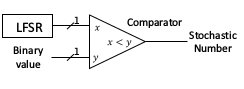
\includegraphics[width=15em]{fig1.png}
        \caption{ Stochastic Number Generator}
    \end{minipage}}   
    \hspace{0px}
    \mbox{\begin{minipage}[b]{0.33\textwidth}
        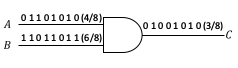
\includegraphics[width=15em]{fig2.png}
        \caption{ An AND gate as a stochastic multiplier}
    \end{minipage}}
    \hspace{0px}
    \mbox{\begin{minipage}[b]{0.33\textwidth}
        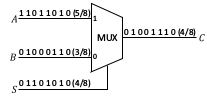
\includegraphics[width=15em]{fig3.png}
        \caption{ Multiplexer used as a scaled stochastic adder}
    \end{minipage}}
\end{figure*}

\begin{figure}[ht]
\begin{center}
    \setcounter{figure}{3}
    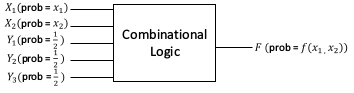
\includegraphics[width=.4\textwidth]{fig4.png}
    \caption{ An SC Circuit by the Method \cite{fifteen}.}
\end{center}
\end{figure}

The framework of the method in \cite{fifteen} to generate an SC circuit to implement a BCP is to design a circuit as shown in Fig. 4. More concretely, in the framework, they consider the following problem.
\smallskip
\fbox {\parbox{0.95\linewidth}{%
       \textbf {SC Circuit Design Problem.} \\
We are given a BCP $f(x_1, x_2, \cdots, x_n)$. Our task is to
design a Boolean function (circuit) $F(X_1, X_2,\cdots, X_n)$
such that the probability of the output F to be 1
is exactly the same as the value of $f(x_1, x_2,\cdots, x_n)$
when $X_1, X_2,\cdots, X_n$ become 1 with probability
$x_1, x_2,\cdots, x_n,$ respectively. We may use some auxiliary Boolean variables whose probabilities to be 1 is known to us.
    }%
 }   


This means that the generated circuit (F) can compute the
output value of $f(x_1, x_2, \cdots , x_n)$ in the SC manner.

\noindent
\underline{\textbf{The method \cite{fifteen} to design a BCP}}
\par
The method [15] can solve the above problem by designing
a circuit (as shown in Fig. 4) such that \\
\begin{itemize}
  \item The circuit has n input SNs, $X_1, X_2, \cdots , X_n$, whose
values are $x_1, x_2, \cdots , x_n,$ respectively.
  \item If $h(a_1, a_2, \cdots , a_n)$ in the above BCP form needs $\frac{1}{2^m}$ precision (i.e., if the value of $h(a_1, a_2, ... , a_n)$ is a multiple of $\frac{1}{2^m}$), we prepare m auxiliary input SNs, $Y_1, Y_2, \cdots , Y_m$, whose values are all $\frac{1}{2}$.
  \item The circuit generates a Boolean function $F(X_1, X_2, \cdots , X_n, Y_1, Y_2, \cdots , Y_m)$ such that the probability of the F to be 1 is exactly the same as the value of the target BCP $f(x_1, x_2, \cdots , x_n)$.

\end{itemize}

\par
How to derive the above Boolean function
$F(X_1, X_2, \cdots , X_n, Y_1, Y_2, \cdots , Y_m)$ is as follows:
the method chooses F such that the number
of combinations $(b_1, b_2, \cdots , b_m)   \:\epsilon\:   \left \{ 0,1 \right \}^m$ that
makes $F(a_1, a_2, \cdots , a_n, b_1, b_2, \cdots , b_m) = 1$ be
$h(a_1, a_2, \cdots , a_n) \times 2^m$ for each $(a_1, a_2, \cdots , a_n) \:\epsilon\:   \left \{ 0,1 \right \}^n$.
There are many candidates of F to satisfy this; their heuristic
to find such F by setting the values of the correspond truth
table (in a simple order) to satisfy the above condition. See
more details in [15] because the heuristic is out of scope of
this paper.

\par
The above choice of F can be justified as follows. When
we fix $(X_1, X_2, \cdots , X_n)$ as $(a_1, a_2, \cdots , a_n) \:\epsilon\:   \left \{ 0,1 \right \}^n$, there are still $2^m$ combinations for the inputs of $(Y_1, Y_2, \cdots , Y_m)$. By the above selection of F, $h(a_1, a_2, \cdots , a_n) \times 2^m$ combinations (out of the $2^m$ combinations) of $(Y_1, Y_2, \cdots , Y_m)$ makes F to be 1. This means that when $(X_1, X_2, \cdots , X_n)$ is $(a_1, a_2, \cdots , a_n)$, the value of F is \\

\begin{math}
\hspace{1cm} \frac{h(a_1, a_2, \cdots , a_n) \times 2^m}{2^m} = h(a_1, a_2, \cdots , a_n).
\end{math}

\noindent
because each $Y_i$ becomes 1 with the same probability $\frac{1}{2}$ and thus each of $2^m$ combinations of ${(Y_1, Y_2, \cdots , Y_m)}$ equally
happens with probability $\frac{1}{2^m}$ .

\par
Note that $X_i$ becomes 1 and 0 with probability $x_i$ and
$(1 - x_i)$, respectively. Thus, the probability of the inputs
$(X_1, X_2, \cdots , X_n)$ to be $(a_1, a_2, \cdots , a_n)$ can be expressed as $\prod_{j=1}^{n}x_j^{a_j}(1-x_j)^{1-a_j}$.  Therefore, the value of $F$ is $\sum_{a_1, a_2,...,a_n\epsilon \{{0,1}\}^{n}}h(a_1, a_2,...,a_n)\prod_{j=1}^{n}x_j^{a_j}(1-x_j)^{1-a_j}$ which is equal to $f(x_1, x_2,\cdots, x_n)$ as desired.

\subsection{A Motivational Example}

Suppose we want to construct a Boolean circuit that realizes
the following BCP: $f(x_1, x_2) =h(0, 0)(1 - x_1)(1 - x_2) +
h(0, 1)(1 - x_1)x_2 + h(1, 0)x_1(1 - x_2) + h(1, 1)x_1x_2$, where
the values of $h(0, 0), \cdots , h(1, 1)$ are given in Table I.

\par
To realize the above BCP, the key task is to produce
stochastic numbers whose values are $\frac{1}
{8}$ , two $\frac{2}{8}$ and $\frac{3}{8}$ at the
same time. To do so, the method \cite{fifteen} needs three auxiliary
input stochastic numbers, $Y_1, Y_2, Y_3$, whose values are equally $\frac{1}{2}$ . This is because we need to generate $\frac{1}{2^3}$ -precision stochastic
numbers. The generated Boolean function by the method \cite{fifteen}
can be shown as in Table II where $X_1$ and $X_2$ are the input
stochastic numbers corresponding to the input variables, $x_1$
and $x_2$ in the given BCP.

\par
Because $Y_i$ = $\frac{1}{2}$ , each minterm with respect to $Y_1$, $Y_2$, $Y_3$
(e.g., $Y_1 \cdot Y_2 \cdot Y_3, \overline{Y_1}\cdot\overline{Y_2}\cdot Y_3$, etc.) can be a stochastic number
whose value is$\frac{1}{8}$ . Thus, if we want to make each of the four
stochastic numbers (corresponding to the values of $h(X_1, X_2)$
in Table I), we just take the same number of minterms as the
numerator of the value of the corresponding $h(X_1, X_2)$. For
example, if we want to generate a stochastic number whose
value is $h(0, 0) = \frac{1}{8}$, we may take two minterms, e.g.,$Y_1\cdot Y_2 \cdot Y_3 + \overline{Y_1}\cdot\overline{Y_2}\cdot Y_3$ We can take any combination of minterms as
long as the number of minterms is the same as the numerator
of $h(X_1, X_2)$.

\par
The paper \cite{fifteen} proposes a heuristic to select minterms in
order to make the resultant Boolean formula simple as follows.
First, we express the target number (i.e., the numerator of
$h(X_1, X_2)$) as the form of $\sum_{k} 2^{k}$. For example, we get the
expression $3 = 2^1 + 2^0$ for the numerator of $h(1, 1) = \frac{1}{8}$ .

\par
Next, for each term $2^k$ in the above expression: $\sum_{k} 2^{k}$,
we construct a product term as follows. When we use m
input stochastic numbers $(Y_i (1 \leq i \leq m))$, a product term
consisting of $(m - k)$ input variables can be a stochastic
number whose value is $2^k$ because the product term does not
have $k$ input variables; it contains $2^k$ minterms.
\smallskip

\begin{table}[t]
    \mbox{\begin{minipage}[b]{0.22\textwidth}
      \caption{COEFFICIENTS OF AN EXAMPLE BCP.}
    \begin{tabular}{c c |c}
    \hline
     $X_1$ & $X_2$ & $h(X_1, X_2)$\\
      \hline
      0 & 0 & $h(0, 0) = \frac{2}{8}$\\
      0 & 1 & $h(0, 1) = \frac{2}{8}$\\
      1 & 0 & $h(1, 1) = \frac{1}{8}$\\
      1 & 1 & $h(1, 1) = \frac{3}{8}$ \\ \hline
    \end{tabular}
    \bigskip
    \bigskip
    \caption{THE GENERATED FUNCTION BY OUR METHOD.}
    \begin{tabular}{c c |c c| c}
    \hline
     $X_1$ & $X_2$ & $Y_1$ & $Y_2$ &$F$\\ \hline
        0 &0 &1 &1 &1\\ 
        0 &0 &0 &1 &1\\ 
        0 &0 &1 &0 &0\\ 
        0 &0 &0 &0 &0\\  \hline
        0 &1 &1 &1 &1\\ 
        0 &1 &0 &1 &1\\ 
        0 &1 &1 &0 &0\\ 
        0 &1 &0 &0 &0\\  \hline
        1 &0 &1 &1 &1\\ 
        1 &0 &0 &1 &0\\ 
        1 &0 &1 &0 &0\\ 
        1 &0 &0 &0 &0\\  \hline
        1 &1 &1 &1 &0\\ 
        1 &1 &0 &1 &0\\ 
        1 &1 &1 &0 &1\\ 
        1 &1 &0 &0 &0\\  \hline
    \end{tabular}
    \end{minipage}}   
    \hspace{5px}
    \mbox{\begin{minipage}[b]{0.22\textwidth}
        \caption{THE GENERATED FUNCTION BY THE METHOD [15].}
        \begin{tabular}{c c |c c c | c} \hline
     $X_1$ & $X_2$ & $Y_1$ &$Y_2$ &$Y_3$ & $F$\\ \hline
        0 &0 &1 &1 &1 &0\\ 
        0 &0 &1 &1 &0 &0\\ 
        0 &0 &1 &0 &1 &1\\ 
        0 &0 &1 &0 &0 &1\\ 
        0 &0 &0 &1 &1 &0\\ 
        0 &0 &0 &1 &0 &0\\ 
        0 &0 &0 &0 &1 &0\\ 
        0 &0 &0 &0 &0 &0\\ \hline
        0 &1 &1 &1 &1 &0\\ 
        0 &1 &1 &1 &0 &0\\ 
        0 &1 &1 &0 &1 &1\\ 
        0 &1 &1 &0 &0 &1\\ 
        0 &1 &0 &1 &1 &0\\ 
        0 &1 &0 &1 &0 &0\\ 
        0 &1 &0 &0 &1 &0\\ 
        0 &1 &0 &0 &0 &0\\ \hline
        1 &0 &1 &1 &1 &0\\ 
        1 &0 &1 &1 &0 &1\\ 
        1 &0 &1 &0 &1 &0\\ 
        1 &0 &1 &0 &0 &0\\ 
        1 &0 &0 &1 &1 &0\\ 
        1 &0 &0 &1 &0 &0\\ 
        1 &0 &0 &0 &1 &0\\ 
        1 &0 &0 &0 &0 &0\\ \hline 
        1 &1 &1 &1 &1 &0\\ 
        1 &1 &1 &1 &0 &1\\ 
        1 &1 &1 &0 &1 &1\\ 
        1 &1 &1 &0 &0 &1\\ 
        1 &1 &0 &1 &1 &0\\ 
        1 &1 &0 &1 &0 &0\\ 
        1 &1 &0 &0 &1 &0\\ 
        1 &1 &0 &0 &9 &0\\ \hline 
    \end{tabular}
    \end{minipage}}
\end{table}
%-------------------------------------------
%-------------------------------------------
%-------------------------------------------
\par
We have a freedom to select $(m-k)$ input variables as well
as whether or not each variable is negated. The heuristic in  \cite{fifteen}
selects a product term: $Y_1 \cdot Y_2 \cdot Y_{m-k-1} \cdot \overline{Y_{m-k}}$ (i.e., we select
from $Y_1$ to $Y_{m-k}$ and only the last variable is negated). For
example, if we want to generate a stochastic number whose
value is ${2}^{m-1}$ (when we use $m$ inputs), we select a product
term: $Y_1$. Also, $Y_1\overline{Y_2}$ can be a stochastic number whose value
is ${2}^{m-2}$.

\par
Therefore, the heuristic generates $h(1, 1) = Y_1 \cdot \overline{Y_2} + Y_1 \cdot
Y_2 \cdot \overline{Y_3}$ in the above example because the numerator of $h(1, 1)$
is $3 =2^0 + 2^1$ and $m = 3$, and so we generate $Y_1 \cdot Y_2$ for $2^1$,
and $Y_1 \cdot Y_2 \cdot Y_3$ for $2^0$. 

\par
For each $2^k$ in the above form:$\sum_{k} 2^{k}$ of the target, we
select a product term as mentioned above. To sum up, we get
the following Boolean formula for each $h(X_1, X_2)$ in Table I:
$h(0, 0) = Y_1 \cdot \overline{Y_2}, h(0, 1) = Y_1 \cdot \overline{Y_2}, h(1, 0) = Y_1 \cdot Y_2 \cdot \overline{Y_3}, h(1, 1) = Y_1 \cdot Y_2 + Y_1 \cdot Y_2 \cdot \overline{Y_3}.$

\par
We can easily see that each of the above $h(X_1, X_2)$ expression
contains the same number of minterms as the numerator
of the corresponding value of $h(X_1, X_2)$ in Table I, and therefore
the above expressions can generate four desired stochastic
numbers at the same time. For example, the probability of the
logic expression: $Y_1 \cdot \overline{Y_2} + Y_1 \cdot Y_2 \cdot \overline{Y_2}$ becomes one is 
$\frac{1}{2} \times \frac{1}{2} + \frac{1}{2} \times \frac{1}{2} \times \frac{1}{2}$
, which becomes $\frac{3}{8}$ , i.e., $h(1, 1)$ indeed.

\par
It seems very natural to use m stochastic numbers (as
inputs) to generate many stochastic numbers of the form $\frac{l}{2^m}$ ($l$
is an integer) at the same time as the method proposed in  \cite{b15}

\par
A bit surprisingly, we will show that there is a method to do
the same task with much fewer stochastic number inputs if we
select the probability of the inputs to be one very carefully. As
we will explain, our proposed construction can produce many
of stochastic numbers of the form $l/2^{\frac{m(m+1)}{2}}$ ($l$ is an integer) at
the same time with only $m$ stochastic inputs. This means that our method needs quadratically smaller number of stochastic number inputs when we want the same precision. For example,
to realize the same BCP, we need only two stochastic number inputs.

\par
As we explain later, our new proposed method can generate
stochastic numbers corresponding to the same h(X1, X2) as
shown in Table I as follows: $h(0, 0) = Y_2, h(0, 1) = Y_2,
h(1, 0) = Y_1 \cdot Y_2, h(1, 1) = Y_1 \cdot Y_2$. In the same way as
mentioned above, it is easy to see that this expression can
produce the probabilities as desired. Thus our method is better
than the method \cite{fifteen} in this example although the difference
is small. We can expect the difference becomes larger when
we need more precisions, i.e., when $m$ is larger.

\par
It should be noted that our method can produce a smaller
circuit to realize the above-mentioned BCP by the conventional
methods as mentioned in Section II-B; we need 6 AND gates
and 3 multiplexers to realize the BCP by a conventional design
method because an multiplication needs one AND gate, and an
addition needs one multiplexer as explained in Section II-B.
On the contrary, our method needs 5 AND gates and 2
multiplexers to realize the same BCP.

\section{ OUR PROBLEM FORMULATION}
\par
In the previous problem called \textbf{SC Circuit Design Problem},
our essential problem is to design an SC circuit whose output
becomes 1 with a certain desired probability. That is, we
want to make an stochastic number corresponding to each
$h(a1, a2, ··· , an)$ in the BCP form. This problem is almost
similar to make an SN from a given set of initial SNs, which
has been studied intensively, e.g, \cite{twelve}. The problem we study
in this paper can be stated as follows:
\fbox {\parbox{\linewidth}{%
       \textbf {Stochastic Number Generation Problem.} \\
We can use (possibly) many input SNs whose values
are known beforehand. (The probability can be different
for different input SNs.) Our problem is to construct a
Boolean circuit whose (possibly many) outputs become
1 with given (independent) target probabilities. Our objective
is to reduce the number of input SNs to be used as
well as the circuit cost (e.g., the number of gates, depth,
etc.)
    }%
 }   

\section{ OUR PROPOSED METHOD: STOCHASTIC NUMBER GENERATION WITH FEW INPUTS}
\par
In this section, we propose an efficient method to solve the
above \textbf {Stochastic Number Generation Problem.} Our method
uses k auxiliary inputs whose values are $\frac{1}{2},\frac{1}{2^2}, \cdots \frac{1}{2^k}, $ unlike the method \cite{fifteen} where all the auxiliary inputs become 1 with
%--------------------Algorithm
%----------------------------
%-----------------------------
\begin{algorithm}
    \caption {$GenFormula(l, i)$: generating a logic formula
    for probability $l/{2^\frac{1}{i(i+1)}}$ by using $Y_1, \cdots , Y_i$.
    }
    \begin{algorithmic}[1]
    \Require
      \Statex $l$: target probability
    \Require
        \Statex$i$: the current variable index
    \If {$i = 0$}
    \State \Return a null string
    \Else  \State $B \gets 2^i-1$
    \State {$a_1$ and $a_2$ \gets Chose two integers $a_1$ and $a_2$ from \linebreak\{ 0,1,\cdots ,$2^\frac{i(i-1)}{2}$ \} such that $l = a_1 + a_2 \times B$ }
    \If{$a_1 = 0$ and $a_2 = 0$}
    \State \Return a null string
    \EndIf
    \If {$a_1 > 0$ and $a_2 = 0$}
    \State \Return $Y_i \cdot GenFormula(a_1, i - 1)$
    \EndIf
    \If {$a_1 = 0$ and $a_2 > 0$}
    \State \Return $\overline{Y_i} \cdot GenFormula(a_2, i - 1)$
    \EndIf
    \If {$a_1 > 0$ and $a_2 > 0$}
    \State \Return $Y_i \cdot GenFormula(a_1, i - 1) + Y_i \cdot GenFormula(a_1, i - 1)$
    \EndIf
    \EndIf
  \end{algorithmic}
\end{algorithm}
the same probability $\frac{1}{2}$ . This is the main idea of our proposed
method, and thanks to the idea our method needs fewer inputs.

\par
For simplicity, we consider that the number of output is
one, but generalization should be very easy; we just apply the
following method to each output one by one.

\par
More precisely, our method can generate a Boolean formula
F with respect to input variables $Y_1, Y_2, \cdots , Y_k$ whose values
are $\frac{1}{2},\frac{1}{2^2}, \cdots \frac{1}{2^k},$ respectively. The values of $F$ can be made
as $l/2^{\frac{k(k+1)}{2}}$ for any integer $l (0 \leq l \leq 2^{\frac{k(k+1)}{2}})$ by our method. Note that the method \cite{fifteen} explained in Section II-C can make
a probability of the form $\frac{l}{2^k}$ for any integer $l (0 \leq l \leq 2k)$
if $k$ auxiliary inputs are used. Thus our method can create
quadratically many kinds of probabilities compared to the
method \cite{fifteen} when the numbers of auxiliary inputs are the
same (i.e.,$2^{\frac{k(k+1)}{2}}$ versus $2^k$ when we use $k$ auxiliary inputs).

\par
A pseudo-code of our proposed method is as shown in
Algorithm 1. As will become clear in the followings, this
algorithm returns a logic formula to generate an SN representing
a desired probability of the form $l/2^{\frac{k(k+1)}{2}}$ with an
arbitrary integer $l (0 \leq l \leq 2^{\frac{k(k+1)}{2}})$. Here we assume we can
use $k$ inputs, $Y_1, Y_2, \cdots , Y_k,$ whose values are $\frac{1}{2},\frac{1}{2^2}, \cdots \frac{1}{2^k},$ respectively. Thus, the formula we get is with respect to
$Y_i$. The algorithm is recursively called; at the i-th recursion
level, $Y_i$ is considered for the logic formula. The algorithm
${GenFormula(l, i)}$ returns a logic formula as a string for representing
the probability $l/2^{\frac{i(i+1)}{2}}$ with respect to $Y_1, \cdots, Y_i.$
Therefore, we first call ${GenFormula(l,k)}$ if we want to make
a logic formula to produce $l/2^{\frac{k(k+1)}{2}}$ by using $k$ inputs.

\par
When we call ${GenFormula(l,i)}$ and if $i > 0$, first we
set B as $2^i - 1$ at line 4. For example, B is set to be 7
when i = 3. Second, we choose two integers $a_1$ and $a_2$ such
that $l = a_1 + a_2 \times B$ at line 5. Then, we further call recursively
${GenFormula(a_1,i-1)}$ and ${GenFormula(a_2,i-1)}$.
These two recursive calls return two logic formula by using
$Y_1, \cdots , Y_{i-1}$ corresponding to two SNs whose values are

\begin{figure}[t]
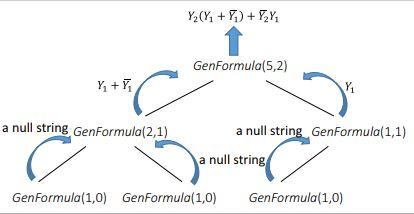
\includegraphics[width=\linewidth]{fig5.png}
\caption{ A Running Example of Our Algorithm.}
\end{figure}

%---------------------------------------------------------Figure%
%--------------------------------------------------------------
%---------------------------------------------------------------
\noindent
$a_1/2^\frac{i(i-1)}{2}$ and $a_2/2^\frac{i(i-1)}{2}$ . Because the probabilities of $Y_i$
and $\overline{Y_i}$ to be 1 are $\frac{1}{2^i}$ and $1 −\frac{1}{2^i} = \frac{B}{2^i}$, respectively, the probability of the logic formula: $Y_i \cdot GenFormula(a_1, i −
1) + \overline {Y_i}\cdot GenFormula(a_2, i−1)$ becomes 1 can be calculated
as: $\frac{1}{2^i}\times a_1/2^\frac{i(i-1)}{2} + \frac{B}{2^i}\times a_2/2^\frac{i(i-1)}{2}.$ This probability should be $l/{2^\frac{1}{i(i+1)}}$ as desired because $l = a_1 + a_2 \times B$. If both $a_1$ and $a_2$ become 0 for $l = 0$, a null string is returned at line 6.
In case of $a_1 > 0$ and $a_2 = 0$, $Y_i$ · ${GenF ormula(a_1, i - 1)}$
is returned at line 9. Choosing $a_2 = 0$ means $ l < B$. When
$a_1 = 0$ and $a_2 > 0$ are selected, $Y_i \cdot GenFormula(a_2, i - 1)$
is returned at line 13. Otherwise, $a_1 > 0$ and $a_2 > 0$, and thus
$Y_i \cdot GenFormula(a_1, i - 1) + Y_i \cdot GenFormula(a_2, i  1)$
is returned at line 15. The recursive calls are performed until
$i = 0$ or $a_1 = a_2 = 0$; a null string is returned in such a case.
It is easy to see that we can finally obtain a logic formula by
this algorithm.

\par
In the following, we explain how the algorithm works by
using an example $(l = 5$ and $k = 2)$ as shown in Fig. 5.
We first call $GenFormula(5, 2)$, and obtain $B = 3$ because
$i = 2$. Next, we choose $a_1$ and $a_2$ such that $l = a_1+a_2\times3$. We
will generate logic formula whose values (we are concerning
only the numerator part for l) are $a_1$ and $a_2$ by the recursive
call with $i = 2$. Thus, $a_1$ and $a_2$ can be in the range from
1 to 2, i.e., $1 \leq a_1, a_2 \leq 2$ because we can generate the
numerators of the probabilities in the above range when we
can use $Y_1$ and $Y_2$. Next we recursively call $GenFormula()$
to generate two logic formula corresponding to a1 and a2.
In this example, $GenFormula(2, 1)$ generates a formula for
a1, and $GenFormula(1, 1)$ generates one for $a_2$. Because the
probability of $Y_2$ and $\overline{Y_2}$ become 1 is $\frac{1}{4}$ and $\frac{1}{4}$, respectively, the formula: $Y_2 \cdot GenFormula(2, 1)+ \overline {Y_2} \cdot GenFormula(1, 1)$ produces a stochastic number such that the numerator of the value of the stochastic number is $1 \times a_1 + 3 \times a_2$, which is our target value. Thus, after getting the two formulas from the recursive calls, we get the above final formula at line 16 in
Algorithm 1.

\par
In the same way, as Fig. 5 shows, $GenFormula(2, 1)$
calls $GenFormula(1, 0)$ and $GenFormula(1, 0)$ because
$a_1$ and $a_2$ are both 1. After getting the result (null
strings) from these recursive calls, we generate the formula:
$Y_1 \cdot GenFormula(1, 0) + \overline{Y_1} \cdot GenFormula(1, 0)$,
which is equal to $Y_1 + \overline{Y_1}$. This formula is is returned
from $GenFormula(2, 1)$ to $GenFormula(5, 2)$ as
Fig. 5 shows. In the same way, $GenFormula(1, 1)$ returns
$Y_1$ to $GenFormula(5, 2)$ as Fig. 5 shows. Finally,
$GenFormula(5, 2)$ combines the two formulas from the
recursive calls to get the final result: $Y_2 ( Y_1 + \overline{Y_1} ) + \overline{Y_2} Y_1 = Y_2 + \overline{Y_2} Y_1.

\par
When $GenFormula(1, 1)$ is called, there are two patterns
choosing $(a_1, a_2) = (1, 0)$ or $(0, 1)$. Indeed, in most cases,
%------------------------- Table ----------------------------%
%--------------------------------------------------------------
%---------------------------------------------------------------
\begin{table}[ht]
     \caption{COMPARISON OF THE TWO METHODS.}
    \begin{tabular}{c|c ||c|c}
    \hline
     Ratio (r) &  # of cases & Ratio (r) & # of cases\\ \hline  
      $1 < r \leq 1.2$ & 2 & $7 < r \leq 9$ & 18 \\
   $ 1.2 < r \leq 1.5$ & 40 & $9 < r \leq 11$ & 4 \\
    $1.5 < r \leq 1.75$ & 153 & $11 < r \leq 13$ & 2 \\
    $1.75 < r \leq 2$ & 209 & r = 1 & 6 \\ 
    $2 < r \leq 3$ & 416 & inf & 6 \\
    $3 < r \leq 5$ &140 &nan & 1 \\
    $5 < r \leq 7$ &26 & & \\ \hline
    \multicolumn{3}{c}{total} & 1023 \\ \hline
    \end{tabular}
\end{table}

the choice of $a_1$ and $a_2$ can be several ways; we may reduce
the final circuit cost by selecting a good choice, which is not
considered in this paper; it should be our future work.

\section{PRELIMINARY EXPERIMENTAL RESULTS}
In this section, we compare our proposed method with the
previous method \cite{fifteen}. It should be noted that the method \cite{fifteen}
and our method will be used to design a circuit to produce
many desired probabilities at the same time as a part of SC
circuits. However, the essential difference between our method
and the previous method \cite{fifteen} is the part of generating Boolean
formula to produce desired probabilities. Thus, to see only this
point clearly, we compare logic formulas by the two methods
to produce a single probability. More precisely, we generated
logic formulas to produce $\frac{l}{1024}$ for all $l (0 < l< 1024)$. This
means we use $k = 4$ inputs for our method, and 10 inputs for
the method \cite{fifteen}. Then we optimized circuits corresponding
to the logic formulas with the standard script “resyn2” of
ABC \cite{five} in order to compare the number of 2-input AND
gates in the corresponding generated circuits. As mentioned
in Section IV, our method can find multiple logic formulas
for the same target probability. In our experiments, we tried
all the formulas to be processed by ABC and report the best
result in the following.

\par
We counted the numbers of 2-input AND gates in the
generated circuits by the two methods; we observed that our
method is always better or equal to the previous method. The
average numbers of gates are 3.48 and 8.92, by our method
and the previous method, respectively. The ratio of the number
of AND gates by the method \cite{fifteen} to that by our method is
always greater or equal to 1. (Note that if this ratio is larger
than one, our method is considered to be better.) The average
of this ratio is 2.75, which means that the previous method
needs 2.75 times more gates than our method in average. The
maximum number of gates by the previous method was 43
whereas the same number for our method is only 5.

\par
In Table IV, we report how many test cases exist for the
different ratios. For example, the second row means that there
are only two cases out of 1,023 cases where the ratio does not
exceed 1.2 (and larger than 1).

\par
In some cases, we do not need a logic gate to produce a
target probability. For example, if we want to produce $\frac{512}{1024}$ , we just use $Y_1$ whose values is $\frac{1}{2}$ , and thus we do not need
any AND gate. If both methods do not need any AND gate,
the ratio is reported as “nan” in the table. If our method does
not need any AND gate but the method \cite{fifteen} needs some gates,
the ratio is reported as “inf” in the table. Also there is 6 cases
when the two methods need the same number of gates; they
are the case when $r = 1$ in the table. Such special cases are
reported in the lower part of the table.
\par
In our experiment, we examined the case where the target
probability is $\frac{l}{1024}$ for all $l (0 <l< 1024)$. Thus our
method and the method \cite{fifteen} need only four and ten inputs, respectively, and so the difference in terms of the number of AND gates may not become so large in many cases. However, when we need more precision for the target probability, we
may need more detailed probability of the form $\frac{l}{2^15}$ . In such a case, our method needs 5 inputs while the method \cite{fifteen} needs
15 inputs, which means that the difference of the numbers of
inputs becomes larger; we can expect our method becomes more advantageous.

\section{CONCLUSION AND FUTURE WORKS}
\par
In this paper, we have proposed a new method to generate
many stochastic numbers for the general design method
of stochastic circuits. Our method needs much fewer input
stochastic numbers than the previous method, and thus our
method can indeed generate smaller circuits than the previous
method for the same purpose. Intuitively, our method needs
the minimum number of necessary input stochastic numbers;
indeed we can prove so although we cannot show the proof
due to the space limit. Such a discussion should be appeared in
our next work. Our obvious remaining task is to study how to
select a good pair of $a_1$ and $a_2$ if there are many candidates in
our proposed algorithm: $GenFormula$. Also, as an important
future work, we need to evaluate many practical stochastic
circuits by using stochastic numbers by our method.

\begin{thebibliography}{}
\bibitem{one} Armin Alaghi and John P. Hayes. A spectral transform approach to
stochastic circuits. In 30th International IEEE Conference on Computer
Design, ICCD 2012, Montreal, QC, Canada, September 30 - Oct. 3,
2012, pages 315–321, 2012.

\bibitem{two} Armin Alaghi and John P Hayes. Survey of stochastic computing. ACM
Transactions on Embedded computing systems (TECS), 12(2s):92, 2013.

\bibitem{three}  Boaz Barak, Ronen Shaltiel, and Eran Tromer. True random number
generators secure in a changing environment. In Cryptographic Hardware
and Embedded Systems - CHES 2003, 5th International Workshop,
Cologne, Germany, September 8-10, 2003, Proceedings, pages 166–180,
2003.
\bibitem{four}  Shekhar Borkar, Tanay Karnik, and Vivek De. Design and reliability
challenges in nanometer technologies. In Proceedings of the 41st annual
Design Automation Conference, pages 75–75. ACM, 2004.

\bibitem{five}   Robert Brayton and Alan Mishchenko. Abc: An academic industrialstrength
verification tool. In Proceedings of the 22Nd International
Conference on Computer Aided Verification, CAV’10, pages 24–40.
Springer-Verlag, 2010.

\bibitem{six} Bradley D Brown and Howard C Card. Stochastic neural computation. i.
computational elements. Computers, IEEE Transactions on, 50(9):891–
905, 2001.

\bibitem{seven}  Peng Li and David J Lilja. Using stochastic computing to implement
digital image processing algorithms. In Computer Design (ICCD), 2011
IEEE 29th International Conference on, pages 154–161. IEEE, 2011.

\bibitem{eight}  Weikang Qian, Xin Li, Marc D Riedel, Kia Bazargan, and David J
Lilja. An architecture for fault-tolerant computation with stochastic
logic. Computers, IEEE Transactions on, 60(1):93–105, 2011.

\bibitem{nine} Weikang Qian and Marc D. Riedel. The synthesis of robust polynomial
arithmetic with stochastic logic. In Limor Fix, editor, DAC, pages 648–
653. ACM, 2008.

\bibitem{ten}  Weikang Qian, Marc D. Riedel, Hongchao Zhou, and Jehoshua Bruck.
Transforming probabilities with combinational logic. IEEE Trans. on
CAD of Integrated Circuits and Systems, pages 1279–1292, 2011.

\bibitem{eleven} Saeed Sharifi Tehrani, Ali Naderi, Guy-Armand Kamendje, Saied
Hemati, Shie Mannor, and Warren J Gross. Majority-based tracking
forecast memories for stochastic ldpc decoding. Signal Processing, IEEE
Transactions on, 58(9):4883–4896, 2010.

\bibitem{twelve} Chen Wang and Weikang Qian. Optimizing multi-level combinational
circuits for generating random bits. In Design Automation Conference
(ASP-DAC), 2013 18th Asia and South Pacific, pages 139–144. IEEE,
2013.

\bibitem{thirteen}  D. Wilhelm and J. Bruck. Stochastic switching circuit synthesis. In
Information Theory, 2008. ISIT 2008. IEEE International Symposium
on, pages 1388–1392, July 2008.

\bibitem{fourteen}  Da Zhang and Hui Li. A stochastic-based fpga controller for an induction
motor drive with integrated neural network algorithms. Industrial
Electronics, IEEE Transactions on, 55(2):551–561, 2008.

\bibitem{fifteen} Zheng Zhao and Weikang Qian. A general design of stochastic circuit
and its synthesis. In Proceedings of the 2015 Design, Automation
& Test in Europe Conference & Exhibition, pages 1467–1472. EDA
Consortium, 2015.

\end{thebibliography}
\bibliographystyle{IEEEtran}


\bibliography{main}


\end{document}